\chapter{Multiple Step Ahead Forecasting of the Disturbance Storm Time Index: The GPNN Model}\label{chapter:dst_msa}

\section{Introduction}

It is widely accepted that solar wind/magnetosphere coupling plays a key role in determining the Earth’s 
geomagnetic state. Under appropriate conditions, this coupling can lead to injection of energetic particles 
into the Earth’s auroral and equatorial plasma currents, leading to geomagnetic storms. The solar wind conditions 
that are effective for creating geomagnetic storms are sustained periods of high-speed solar wind and a southward 
directed solar wind magnetic field \citep{JGR:JGR10260}. When \citet{1981AkasofuE} studied the coupling function 
between the solar wind and geomagnetic disturbances, they observed that during these extreme events, the key process 
is magnetic reconnection \citep{magneticreconnection}. Magnetic reconnection produces an enhancement of particle flux 
which creates a depression of the horizontal component of the Earth’s magnetic field and an intensification of the 
westward ring current circulating the Earth \citep{JGRA:JGRA11775}. When there is a geomagnetic storm, the energy 
content of the ring current increases. This increase is inversely proportional to the strength of the surface magnetic 
field at low latitudes. To assess the severity of geomagnetic storms, the Disturbance Storm Time index (Dst index) is 
often used. 

The Dst index \citep{Sugiura1964} is based on measurements from four low latitude stations and 
represents the axis-symmetric magnetic signature of magnetosphere currents (such as the ring current, 
the tail currents and the Chapman-Ferraro current). It is computed using 1-hour average values of the 
horizontal component of the Earth’s magnetic field and is expressed in nano Tesla (nT). In the case of a 
typical magnetic storm, three phases are observed according to Dst variations. First, there is a sudden drop 
corresponding to the storm commencement. Second, the value of Dst stays in its excited state as the ring current 
intensifies (the main phase). Finally, once the z-component of the Interplanetary Magnetic Field (IMF) turns 
northward, the ring current begins to recover and rises back to its quiet level (recovery phase). 

Geomagnetic indices like Dst, Kp, AE and others are used in space weather to describe effects of the solar wind on 
the Earth's magnetosphere. It has been long observed that strong geomagnetic storms disrupt man-made systems, 
they can impact satellites, disrupt navigation systems and create harmful geomagnetic induced currents in power grids 
and pipelines. One of the important research problems in space weather is to predict geomagnetic disturbances, 
in order to protect technological infrastructure \citep{Singh2010}. The aim of this study is to propose an 
accurate and reliable probabilistic model to predict Dst from one hour to six hours ahead. 

The Dst prediction problem has been extensively researched. \citet{JGR:JGR10260} developed a model 
that expressed the time evolution of Dst as an Ordinary Differential Equation (ODE). This method takes into account 
the particle injection from the plasma sheet into the magnetosphere and expresses it based on the solar wind speed, 
density and on the north-south magnetic component of the IMF ($B_z$). \citet{Iyemori1979} used a linear filtering 
prediction method to connect Dst and the southward component of the interplanetary magnetic field. The linear 
assumption, however, has limitations since  the solar wind and magnetosphere form a coupled non-linear system. 

To model nonlinear behavior of magnetospheric response, various models have been proposed. A popular approach 
used to model nonlinear systems is based on artificial neural networks (ANN) \citep{haykin1994neural}. One of the 
earliest models of Dst prediction based on ANNs is due to \citet{lundstedt1994prediction}. They developed 
a feedforward neural network to predict Dst one hour ahead, using $B_z$, the density and the velocity of 
the solar wind. This model was able to model the initial and main phases of geomagnetic storms well, but 
the recovery phase was not modeled accurately. \citet{gleisner1996predicting} developed a time delay 
neural network \citep{Waibel1989} to predict Dst one hour ahead using the proton density, solar wind 
velocity and $Bz$. This approach managed to improve the prediction of storm recovery phases, showing 
the benefits of using the time history of solar wind inputs. \citet{wu1997geomagnetic} used an Elman 
recurrent network \citep{elman} to provide forecast of the Dst index from one hour to six hours ahead. 
Subsequently, \citet{Lund} used the Elman network architecture to provide an operational forecast of 
the Dst index one hour ahead with improved performance. \citet{JGRA:JGRA17461} used a recurrent network, 
to provide an operational forecast of the Kp index. The success of these operational models demonstrate that 
recurrent networks are quite useful in the empirical modelling of magnetospheric response to solar wind drivers. 

Another approach which is at the intersection between physical models and neural networks is provided by 
\citet{Bala2012}. Their approach is based on ANNs and uses the so called Boyle index which represents 
the steady state polar cap potential, as an input. The Boyle index is a combination of the velocity of 
the solar wind, the magnitude of the IMF and the IMF clock angle. It is used to predict Kp, Dst and AE, 
and provides good performance to predict them from one to six hours ahead. \citet{Lazzus} use 
Particle Swarm Optimization (PSO) \citep{eberhart1995new}, instead of the backpropagation algorithm 
\citep{rummelhart1986parallel}, to learn the ANN connection weights. Results obtained in this study show 
that PSO can provide benefits for training Dst prediction models.

\citet{ChandorkarDst} pointed out that various techniques have been used to predict Dst, but do not 
focus on providing probabilistic predictions. Their model is based on \emph{Gaussian processes} (GP) to construct 
autoregressive models to predict Dst one hour ahead, based on a time history of Dst, solar wind velocity and 
the IMF $B_z$. \citet{ChandorkarDst} show that it is possible to generate an accurate predictive distribution 
of the forecast instead of a single point prediction. This is important in the space weather domain where 
operators require error bars on predictions. However, the mean value of the forecast does not yield a 
performance as accurate as the one provided by ANN. 

All the models discussed above are based either on solar wind parameters and past values of Dst. One of the most 
striking features of the Dst index is the link between Dst variation, and the impact on GPS satellites. 
It is widely known that when there is a geomagnetic storm, the quality of the GPS signal is disturbed 
\citep{astafyeva2014geomagnetic}. The magnetic field measured onboard GPS satellites might be key information 
when an important storm occurs \citep{morley2017energetic}. Recently, GPS data has been publicly released under 
the terms of the \emph{executive order for coordinating efforts to prepare the nation for space weather events} 
(\url{https://obamawhitehouse.archives.gov/the-press-office/2016/10/13/executive-order-coordinating-efforts-prepare-nation-space-weather-events}). 

In this work, we propose a technique which combines the predictive capabilities of an ANN with the advantage of the 
probabilistic forecast provided by a GP. We use the so called \emph{long short-term memory network} (LSTM) 
\citep{hochreiter1997long} to provide a single point prediction of the Dst geomagnetic index from one to six 
hours ahead. The prediction produced by the LSTM is used as the mean function of a GP, to obtain a 
probabilistic forecast. We call this hybrid model the \emph{Gaussian Process Neural Network} (GPNN). 
Input parameters of the GPNN are solar wind parameters (density, velocity,  
\( IMF  \vert B \vert  \)  and \(  Bz \) ), six hour time history of Dst, and the magnetic field 
measured onboard GPS satellites. To the best of our knowledge, the LSTM architecture has never 
been used in space weather applications before.

The remainder of this chapter is organised as follows: section \ref{sec:data} presents the data used in this study, 
section \ref{sec:methodgpnn} describes the computational method, how the LSTM and its combination with the GP are 
developed and optimised. Section \ref{sec:resultsgpnn} presents the performance of the LSTM model when producing 
point predictions for the Dst one to six hours ahead, and the evaluation of the probabilistic forecasts provided 
by the GPNN model. 

\section{Data}\label{sec:data}

\begin{figure}
	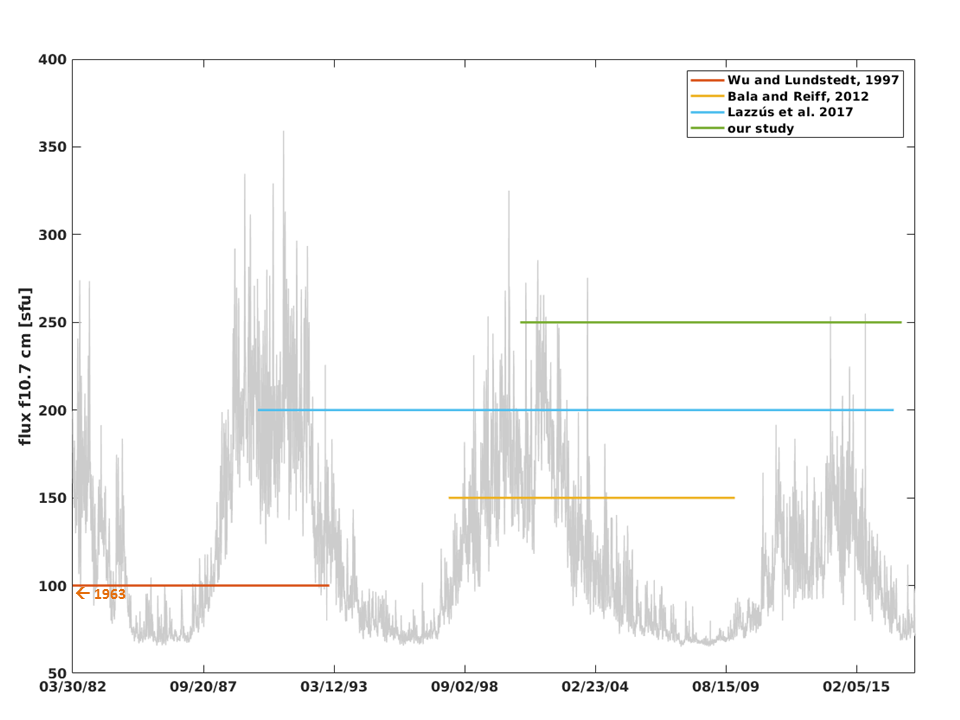
\includegraphics[width=\textwidth]{image2.png}
	\caption{Temporal coverage of database used in this study and in previous studies. \citet{wu1997geomagnetic} 
	is in orange and their database starts in 1963, \citet{Bala2012} is in yellow, \citet{Lazzus} is in blue, and our study is in green. 
	The f10.7 in grey represents the variation of solar activity.}
	\label{fig:datacoverage}
\end{figure}


Solar wind parameters and the geomagnetic Dst index are taken from the OMNI database 
(\url{https://omniweb.gsfc.nasa.gov/ow.html}) maintained by the National Space Science Data Center (NSSDC) 
of National Aeronautics and Space Administration (NASA).

We also consider GPS data which are provided by the National Oceanic and Atmospheric Administration (NOAA). 
This dataset was provided by the team working on the Combined X-ray dosimeter or CXD at the 
Los Alamos National Laboratory (\url{https://www.ngdc.noaa.gov/stp/space-weather/satellite-data/satellite-system/gps/}). 
In this study, we decided to use data recorded by the GPS satellite ns41, which has the widest temporal coverage 
\citep{morley2017energetic}. 

Figure \ref{fig:datacoverage} shows the temporal coverage of the database used in this study, compared to 
previous studies. The temporal coverage of our study is represented by the green line. As GPS ns41 data 
starts at 00:00 14 January 2001, we consider a set of 134,398 hourly data points consisting of 
solar wind parameters, geomagnetic Dst index and GPS data between this starting date and 23:00 31 December 2016. 
This includes 49 storm events, listed in Table \ref{table:teststormsgpnn}. Some of these events in table 
\ref{table:teststormsgpnn} also overlap with events included in \citet{Ji2012} and \citet{ChandorkarDst}. 

Studies done in the past to predict the geomagnetic index Dst have shown that various solar wind parameters 
are of interest when improving performance of Dst models. In the present study, we focused on the use 
of the solar wind density  \( n \) , velocity  \( V \) , the IMF \( \vert B \vert  \) and its  \( B_{z} \) component. 
Concerning parameters provided by the GPS ns41, we use the magnetic field measured by the GPS, \( Bsat_{\text{gps}} \) .

\section{Methodology}\label{sec:methodgpnn}


\subsection{Long Short-Term Memory Network}\label{sec:lstmcomponent}

The \emph{long short-term memory} network (LSTM) belongs to the family of \emph{recurrent neural networks} (RNN). 
In an RNN, hidden layers are built to allow information persistence. They behave as a loop to allow information 
to be passed from one cell of the network to the next. When this loop is unrolled, the RNN can then be thought 
as multiple copies of the same network. The RNN architecture is particulary suited for time series forecasting 
applications. 

\citet{hochreiter1991untersuchungen,bengio1994learning} underlined a weakness of RNNs. They are supposed to connect 
past information to the present, but if the information needed is too far in the past, RNNs are unable to to retain it. 
This failure is due to the so called \emph{vanishing gradient problem} occuring during the training of RNNs. 

LSTM networks are designed to overcome the vanishing gradient problem by retaining information pertaining to long range 
temporal dependencies in time series data. LSTMs have a chain-like structure like RNNs, but the repeating module 
known as the LSTM cell has specific characteristics.

Figure \ref{fig:lstmcell} shows the computational graph of the LSTM cell. The two elements 
fundamental to this cell are the cell state and gates. The cell state $\mathbf{c}_{t}$ in figure \ref{fig:lstmcell} 
is like a conveyor belt which is connected to various gates. Gates can add or remove information from the cell 
state depending on the information required by the LSTM unit. The important pieces of this architecture are: 
\begin{itemize*} 
	\item the forget gate $\mathbf{f}_t$ 
	\item the input gate $\mathbf{i}_t$ 
	\item the cell state $\mathbf{c}_t$ 
	\item the output gate $\mathbf{o}_t$  
\end{itemize*}  

\begin{figure}
	\noindent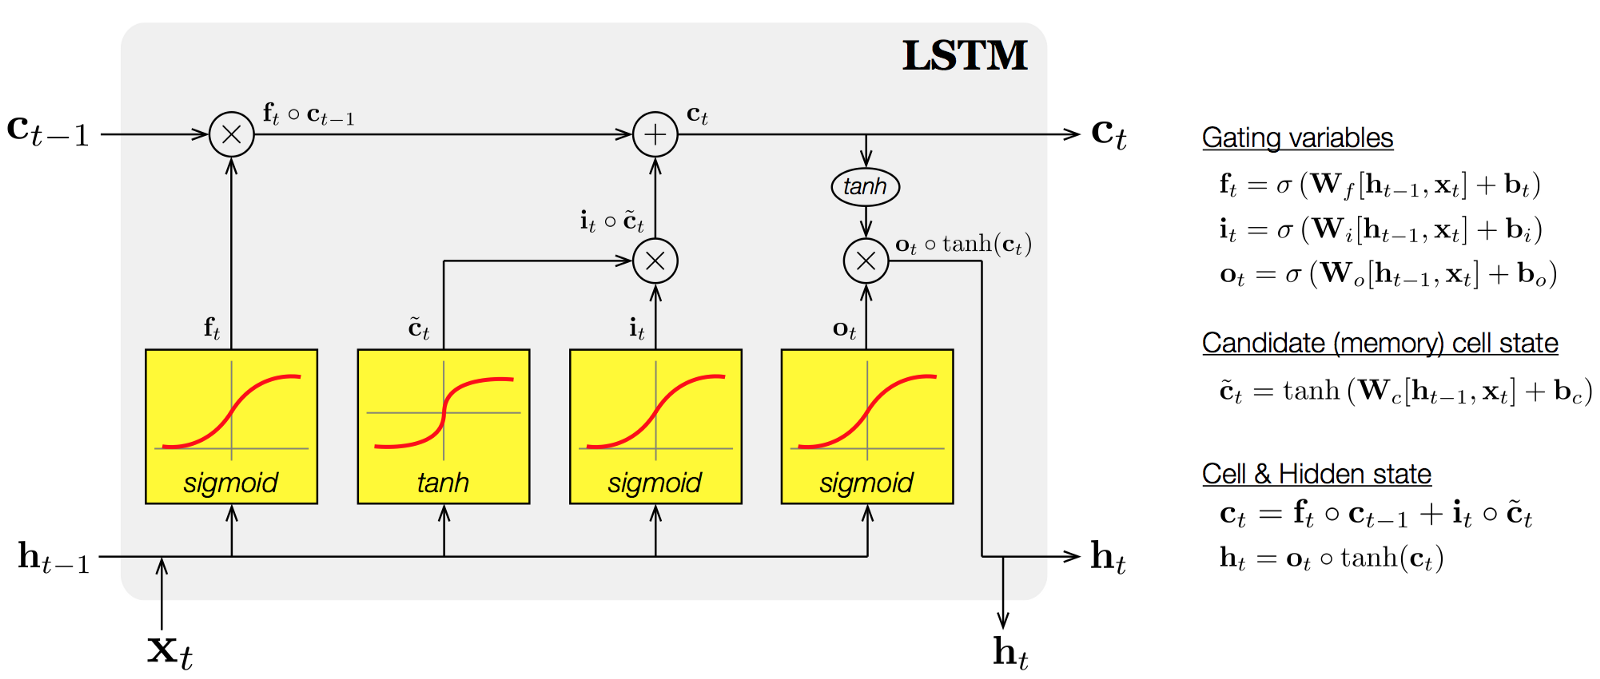
\includegraphics[width=\textwidth]{lstm.png}
	\caption{Schematic diagram of the LSTM cell. Reproduced 
	from \url{https://github.com/llSourcell/LSTM_Networks/blob/master/LSTM\%20Demo.ipynb}}
	\label{fig:lstmcell}
\end{figure}

\subsubsection*{Forget Gate \& Input Gate}

The forget gate is shown in equation \ref{eq:forgetgate}. 

\begin{equation}\label{eq:forgetgate}
 \mathbf{f}_{t} = \sigma  \left( \mathbf{W}_f \boldsymbol{\cdot}  \left[ \mathbf{h}_{t-1}, \mathbf{x}_t \right] + 
 \mathbf{b}_f \right)
\end{equation}

\vspace{\baselineskip}

With  \(  \sigma  \)  the component wise sigmoid function, and  \( \mathbf{W}_{f} \) \  and  
\( \mathbf{b}_{f} \) the weight matrix and bias vector of the gate respectively. This notation is 
kept for subsequent equations. The forget gate compares the information coming from the previous 
cell  \( \mathbf{h}_{t-1} \) and the incoming information  \( \mathbf{x}_{t} \)  and outputs a number 
between zero and one, zero if the information is entirely discarded, one if it is altogether retained.

Correspondingly the input gate (equation \ref{eq:inputgate}) decides what information is retained, depending 
on past hidden cell state $\mathbf{h}_{t-1}$ and exogenous inputs $\mathbf{x}_t$. \( \mathbf{W}_{i} \)  and  
\( \mathbf{b}_{i} \) \ are the weight matrix and bias vector of the input gate respectively.

\begin{equation}\label{eq:inputgate}
 \mathbf{i}_{t} = \sigma  \left(\mathbf{W}_{i} \boldsymbol{\cdot} \left[ \mathbf{h}_{t-1}, \mathbf{x}_{t} \right] + 
 \mathbf{b}_{i} \right)
\end{equation}

\subsubsection*{Cell State}

The inputs $\mathbf{x}_t$ and cell hidden state $\mathbf{h}_{t-1}$ is then passed through a hyperbolic tangent 
transformation create a vector of candidate values \(  \tilde{\mathbf{c}}_{t} \) as per equation \ref{eq:candidate}. 
This candidate state $\tilde{\mathbf{c}}_{t}$ is used to determine the updated cell state $\mathbf{c}_{t}$. 
\( \mathbf{W}_{c} \)  and  \( \mathbf{b}_{c} \)  being the weight and bias of this layer respectively. 
 

\begin{equation}\label{eq:candidate}
 \tilde{\mathbf{c}}_{t} = \text{tanh} \left( \mathbf{W}_{c} \boldsymbol{\cdot}  \left[ \mathbf{h}_{t-1},\mathbf{x}_t \right] + 
 \mathbf{b}_{c} \right)
\end{equation}

The cell state  \( \mathbf{c}_{t-1} \) is then updated to obtain the new cell state \( \mathbf{c}_t \). This 
is shown in equation \ref{eq:newstate}, where $\circ$ denotes the element wise (Hadamard) product. 

\begin{equation}\label{eq:newstate}
 \mathbf{c}_t = \mathbf{f}_{t} \circ \mathbf{c}_{t-1} + \mathbf{i}_{t} \circ \tilde{\mathbf{c}}_{t}
\end{equation}

\subsubsection*{Output Gate \& Prediction}

The output of the LSTM cell is calculated using equation \ref{eq:outputgate}. First, the 
sigmoid transformation helps to define the output $\mathbf{o}_t$. Second, the hidden state $\mathbf{h}_t$ 
is computed by multiplying $\mathbf{o}_{t}$ with a hyperbolic tangent transformation of the cell state 
$\mathbf{c}_{t}$. 

$\mathbf{h}_{t}$ (seen in figure \ref{fig:lstmcell}) becomes the prediction computed LSTM cell and the input 
for the next cell.


\begin{align} \label{eq:outputgate}
	\mathbf{o}_{t} &= \sigma \left( 
		\mathbf{W}_o \boldsymbol{\cdot} \left[\mathbf{h}_{t-1}, \mathbf{x}_{t} \right] + \mathbf{b}_o \right) \\
	\mathbf{h}_{t} &= \mathbf{o}_{t} \circ \text{tanh}(\mathbf{c}_t)
\end{align}

We trained 6 LSTM models corresponding to Dst forecasts from one to six hours ahead. This was implemented using the 
Lasagne library in Python (\url{http://lasagne.readthedocs.io/en/latest/index.html}). We thus obtained a 
vector of outputs \( \textbf{m}_{\text{NN}} \left( \mathbf{x} \right)  = [m^{i}_{\textbf{NN}}(\mathbf{x}); \ i = {1, \cdots, 6}] \), 
for every input \( \mathbf{x} \), which serves as the mean function for the Gaussian process component outlined 
in section \S~\ref{sec:gpcomponent}. 

\subsection{Training of the LSTM}


The LSTM architecture can be trained with a backpropagation based optimization algorithm and thanks to 
its architecture, the vanishing gradient problem does not persist. A number of stochastic gradient based 
variants are used for training neural networks, such as but not limited to \emph{Levenburg - Maquardt} 
\citep{marquardt1963algorithm}, \emph{Nesterov Accelerated Gradient} (NAG) \citep{nesterov1983method}, 
adaptive learning rates for each network weight \citep{SilvaAlmeida}, adaptive gradient based methods such as 
AdaGrad \citep{duchi2011adaptive}, adaptive learning rate methods like RMSprop \citep{tieleman2012lecture}. 

In this work, we use the RMSProp algorithm for training the LSTM component of the GPNN model, below we give 
a brief explaination of its functioning.

\subsubsection*{The RMSProp Algorithm}

For the purposes of notational simplicity, the weights and biases of the LSTM cell are concatenated into a 
single vector $\mathbf{\theta}$, where $\theta_i$ denotes an individual scalar element of $\mathbf{\theta}$. 
We then define \( g_{t,i} \) in equation \ref{eq:gradient} as the gradient of the objective function with respect 
to the parameters \(   \theta_{i} \) at time step t. 

\begin{equation}\label{eq:gradient}
 g_{t,i} = \triangledown_{ \mathbf{\theta} } J \left(  \theta_{t,i} \right)
\end{equation}

The update of parameters using RMSprop is described by equation \ref{eq:learningrmsprop}. First the running average 
of the second order moment of the gradients \( E \left( g^{2} \right)  \) is computed at each iteration $t$, then 
the updated parameters $\theta_{t+1,i}$ are calculated using the gradient $g_{t,i}$ and a damped learning rate of 
$\frac{\eta}{\sqrt{E \left[ g^{2} \right]_{t,i}} + \epsilon }$ ($\epsilon$ is a small number added to 
$\sqrt{E \left[ g^{2} \right]_{t,i}}$ preventing numerical overflow).


\begin{align}\label{eq:learningrmsprop}
 E \left( g^{2} \right)_{t+1,i} &= 0.9 E \left( g^{2} \right)_{t,i} + 0.1 g_{t,i}^{2}  \\ 
 \theta_{t+1,i} &= \theta_{t,i} - \frac{ \eta }{\sqrt[]{E \left[ g^{2} \right]_{t,i}} + \epsilon } g_{t,i}
\end{align}


\subsubsection*{LSTM Model Evaluation}

For the purposes of training and evaluation, the data set is divided as follows : 70$\%$ for training, 20$\%$  
for testing and 10$\%$ for validation. The LSTM model is evaluated using the Root Mean Square Error (RMSE) 
and the Correlation Coefficient (CC) defined by equations \ref{eq:rmse} and \ref{eq:cc} respectively. 


\begin{equation}\label{eq:rmse}
 RMSE = \sqrt[]{ \sum_{t=1}^{n} \left( Dst \left( t \right) - \hat{D}st \left( t \right)  \right) ^{2}/n}
\end{equation}

\begin{equation}\label{eq:cc}
 CC = \frac{Cov \left( Dst, \hat{D}st \right)}{\sqrt[]{Var \left( Dst \right) Var \left( \hat{D}st \right)}} 
\end{equation}


\subsection{Gaussian Processes}\label{sec:gpcomponent}

% \begin{equation}\label{eq:gp}
%  f \left( x \right)  \sim  \mathcal{GP} \left( m \left( x \right) , k \left( x,x' \right)  \right) 
% \end{equation}

% \begin{equation}\label{eq:meanfunc}
%  m \left( x \right) = \mathbb{E} \left[ f \left( x \right)  \right]
% \end{equation}

% \begin{equation}\label{eq:kernelfunc}
%  k ( x,x') = \mathbb{E} \left[  \left( f \left( x \right) -m \left( x \right)  \right)  ( f ( x' ) -m ( x') )  \right]
% \end{equation}

Gaussian processes are a family of models which provide a principled probabilistic framework for forecasting.
GP models output a predictive distribution instead of a point forecast. Starting from a \emph{prior distribution},
GP models construct a \emph{posterior predictive distribution} . The appeal of using GP models is that, even though 
their theoretical formulation might seem rather abstract, the practical implementation is rather straightforward, 
boiling down to simple analytical expression that requires no more than linear algebra. 

We will not give a complete review of the GP methodology here , the interested reader can refer to 
section \S~\ref{sec:osaGPmethod} for a detailed review of Gaussian process models and their mathematical formulation.

A GP is completely specified by its mean function  \( m \left( \mathbf{x} \right)  \) and its covariance function  
\( K (\mathbf{x}, \mathbf{x}') \)  in equation \ref{eq:gpformulation}. 

The covariance function specifies how exactly each point influences the values that the other points are 
likely to take on. The main idea is that if  \( x_{i} \) and  \( x_{j} \)  are close by, 
we expect the output from the functions at these points to be similar . Different types of covariance 
functions exist, also called kernels, which determine the form of the model. 

\citet{ChandorkarDst} listed common kernels used in machine learning and described how the choice of 
it is fundamental. In this study, we focused on the neural network kernel \citep{williams1998computation} 
described in equation \ref{eq:gpcov}. 


\begin{equation}\label{eq:gpcov}
 K_{\text{NN}} \left( \mathbf{x}, \mathbf{x}' \right) = 
 \frac{2}{ \pi } \text{sin}^{-1} \left( \frac{2\mathbf{x}\boldsymbol{\cdot}\mathbf{x}'}{
	 \sqrt{ \left( 1+2\mathbf{x}\boldsymbol{\cdot} \mathbf{x} \right) }\sqrt{ \left( 1+2\mathbf{x}'\boldsymbol{\cdot}\mathbf{x}' \right)}
	 } \right)
\end{equation}


As \citet{Rasmussen:2005:GPM:1162254} described, if there is no prior knowledge about 
the function to be approximated, the mean function is defined to be zero. The aim of our study here is to 
combine the neural network and the gaussian process to obtain accurate forecast with an uncertainty distribution. 
Hence, the mean function  \( m \left( \mathbf{x} \right)  \)  is provided by the  \( \textbf{m}_{\text{NN}} \left( \mathbf{x} \right)  \)  
function described in section \S~\ref{sec:lstmcomponent}.



% \begin{equation}\label{eq:jointdist}
%   \left[ \begin{array}{ll}
% 	f\\
% 	f_{\ast}\\
% 	\end{array} \right] = \mathcal{N}   \left(  \left[ \begin{array}{ll}
% 	m \left( x \right) \\
% 	m \left( x_{\ast} \right) \\
% 	\end{array} \right] ,  \left[ \begin{matrix}
% K \left( X,X \right)   &  K \left( X,X_{\ast} \right) \\
% K \left( X_{\ast},X \right)   &  K \left( X_{\ast},X_{\ast} \right) \\
% \end{matrix}
%  \right]  \right) 
% \end{equation}



% \begin{align}\label{eq:preddist}
%  f_{\ast} \vert X_{\ast},X,f &\sim N \left( f_{\ast},cov \left( f_{\ast} \right)  \right)  \\ 
%  f_{\ast} &= m \left( x_{\ast} \right) +K \left( X_{\ast},X \right)  \left[ K \left( X,X_{\ast}  \right)  \right] ^{-1} \left( y-m \left( x \right)  \right) \\ 
%  cov \left( f_{\ast} \right) &= K \left( X_{\ast},X_{\ast} \right) -K \left( X_{\ast},X \right)  \left[ K \left( X,X \right)  \right] ^{-1} K \left( X,X_{\ast} \right) 
% \end{align}


To predict the geomagnetic index Dst based on input features \( x \) , the equation \ref{eq:dstgp} sumarises 
the inherent process. 



\begin{align}\label{eq:dstgp}
Dst \left( t+p \right) &= f_{p} \left( \mathbf{x}_{t} \right) + \epsilon \\ 
\epsilon &\sim N \left( 0, \sigma ^{2} \right)  \\
f_{p} \left( \mathbf{x}_{t} \right)  &\sim GP \left( m^{p}_{\text{NN}}(\mathbf{x}) , K_{NN}(\mathbf{x}_{t}, x_{s} ) \right)
\end{align}

With  \( p \)  being the expected time forecast. Here we consider $p  = {1,2,3,4,5,6}$ to provide 
multi-step ahead prediction of the Dst index from 1h to 6h ahead. The GP component is implemented using the 
Matlab Software GPML \citep{rasmussen2010gaussian}.


\section{Results} \label{sec:resultsgpnn}


\subsection{Optimisation of the LSTM}


The first step in the development of the GPNN model is to optimise the performance of each 
LSTM to provide predictions of Dst from 1h to 6h ahead. To train LSTM, we use solar wind data and 
GPS data described in section 2 (the density \(  n \) , the velocity  \( V \) , the  
\( IMF  \vert B \vert  \) , its  \( B_{z} \)  component and the magnetic field measured 
by the GPS ns41,  \( Bsat_{\text{gps}} \) ).\ We also use the past history of Dst, from 1h  to 6h back. 
This is summarised with the equation \ref{eq:dstmodel}.



\begin{equation}\label{eq:dstmodel}
	\begin{aligned}
		Dst \left( t+p \right)_{NN} = NN ( 
			& n \left( t \right) , V \left( t \right) , IMF \vert B \vert  \left( t \right) ,Bz \left( t \right) , Bsat_{\text{gps}} \left( t \right) , \\ 
			&	Dst \left( t-1 \right) ,Dst \left( t-2 \right) , \ldots ,Dst \left( t-6 \right) )
	\end{aligned}
\end{equation}

To find the LSTM structure which is the most suitable for predicting geomagnetic storms, we train it 
using various number of cells. The optimal number is 20 and after training, testing and validating each 
LSTM, we compare their performance to neural network models proposed in the past to predict Dst. 
Figures \ref{fig:lstmCC} \ref{fig:lstmCC} presents a  comparison of correlation coefficient and root mean square error 
between our model, with and without using GPS data, and previous models predicting Dst based on NN. 
The temporal coverage of these previous studies are shown in Figure \ref{fig:datacoverage} so the reader 
can have an estimation of the storm times used in them. 

\begin{figure}
	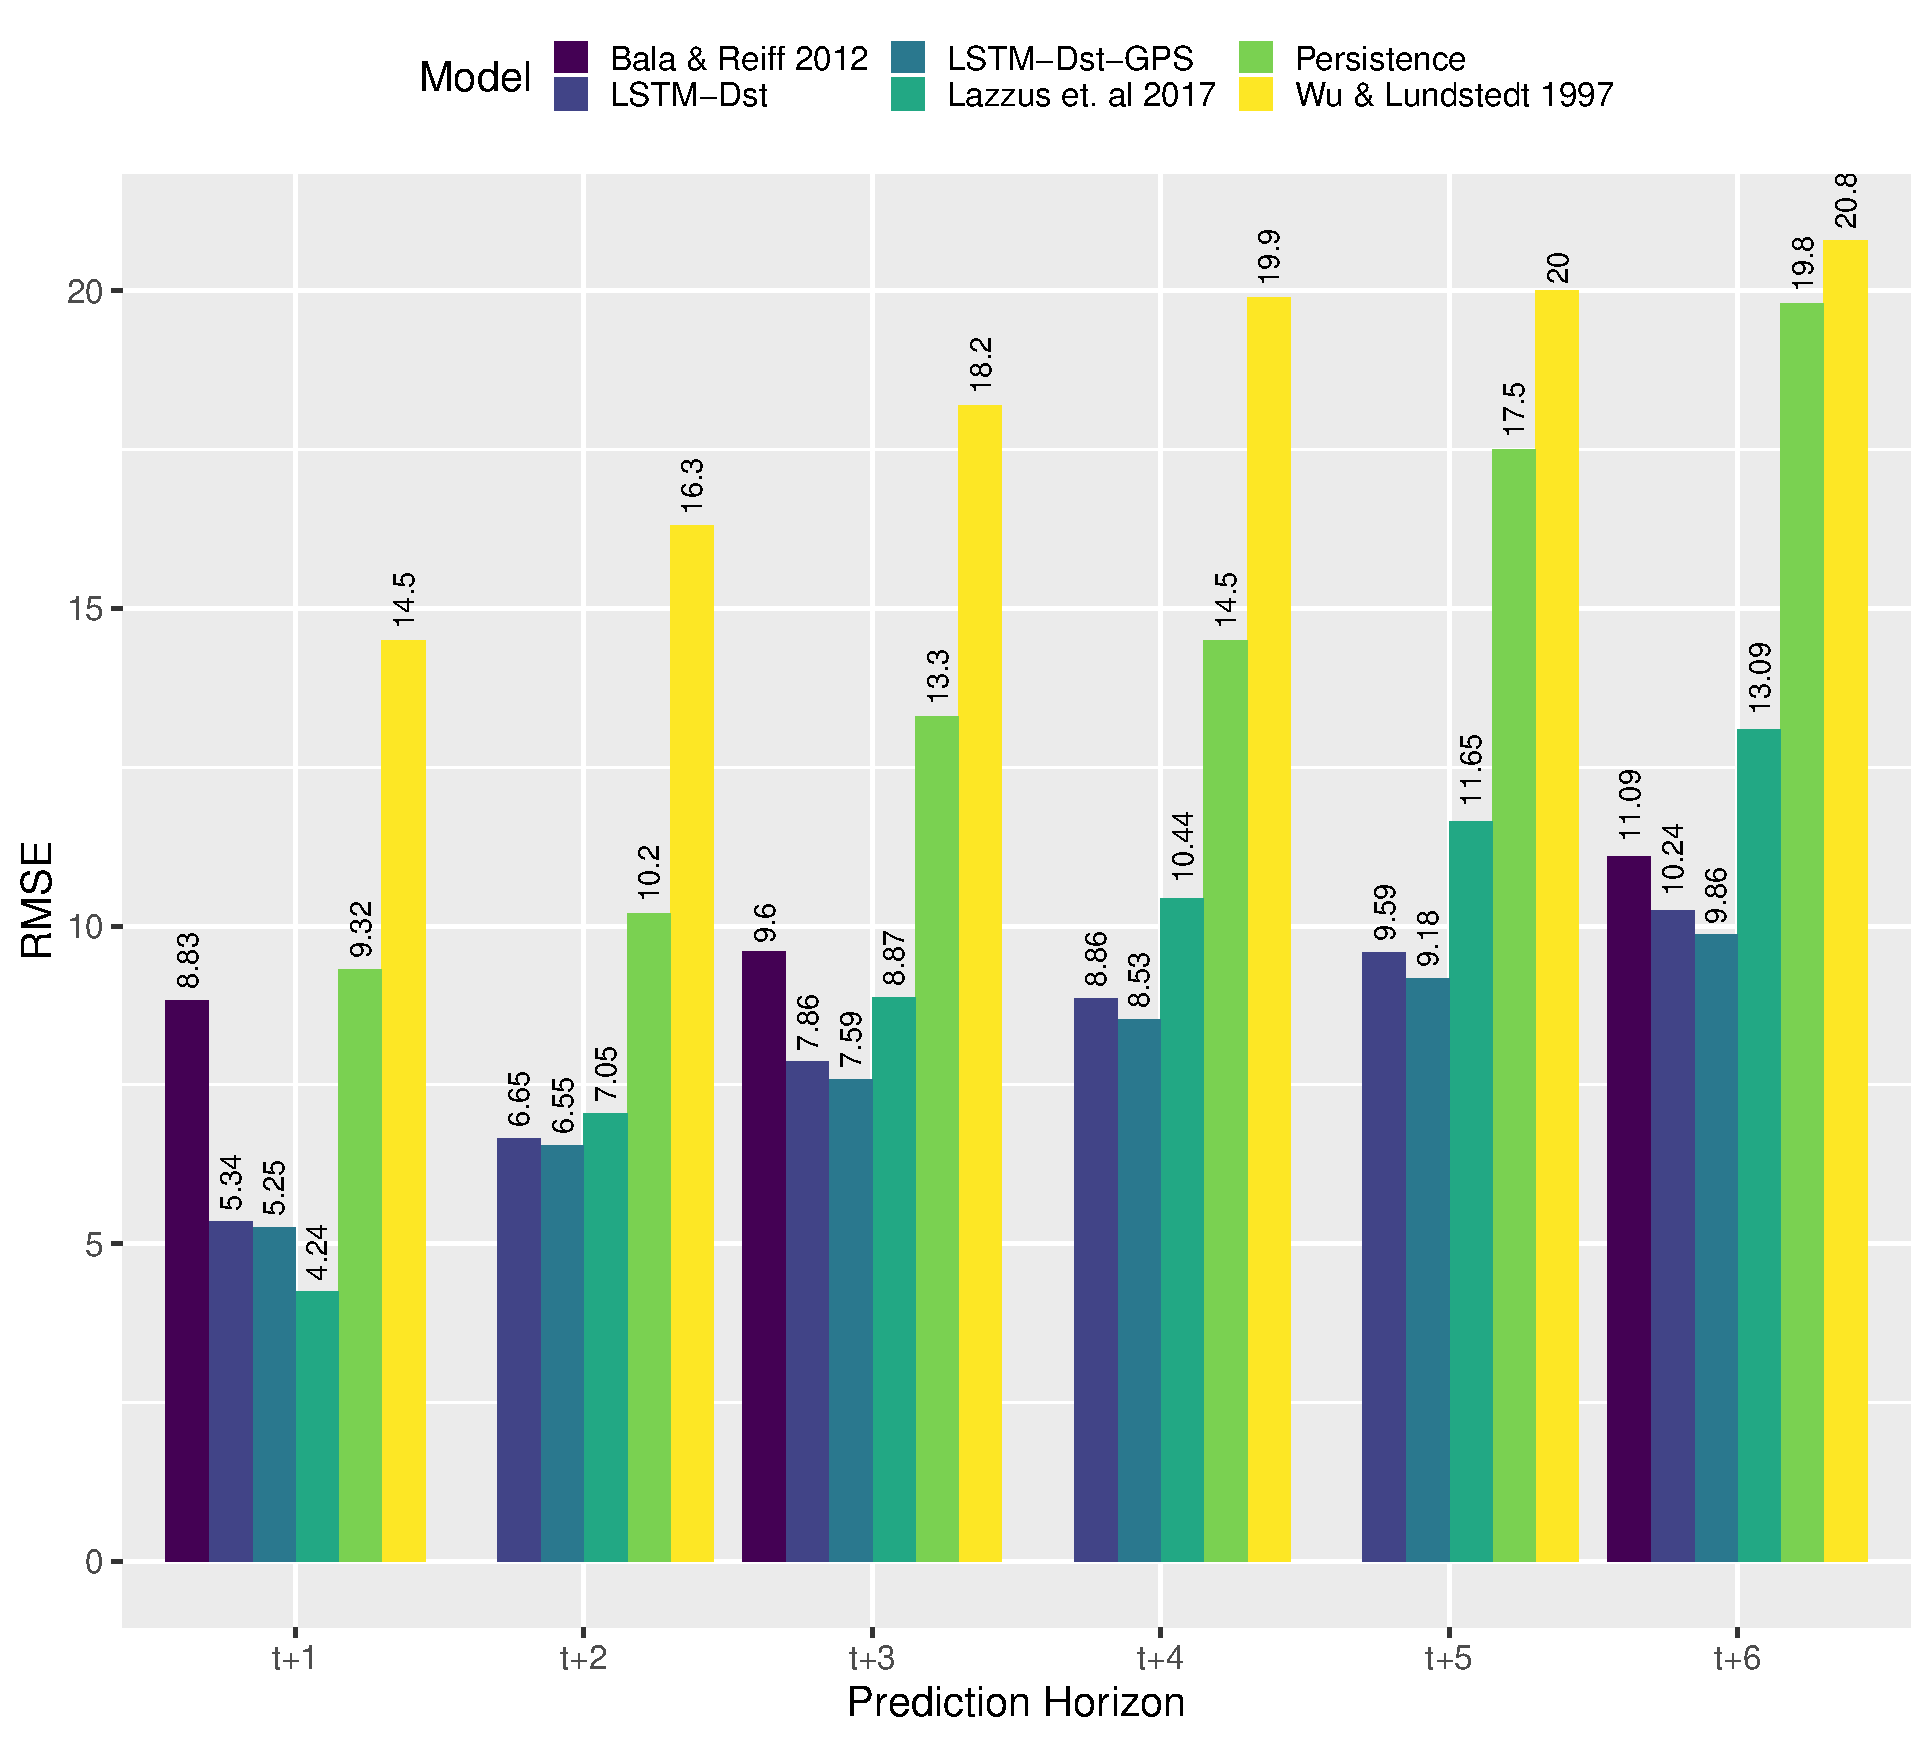
\includegraphics[width=\textwidth]{lstmCompRMSE.pdf}
	\caption{Comparison of RMSE of $Dst$ forecast models.}
	\label{fig:lstmRMSE}
\end{figure}





Our model, with or without GPS data provides performance which are close to the one obtained by 
\citet{Lazzus} from 1h ahead to 3h ahead but when the expected forecast goes from 4h ahead to 6h ahead, 
our models, with or without GPS data provide better global performance. As an example, when considering a 6h 
ahead forecast, our model with GPS data provides a CC of 0.873 and a RMSE of 9.86, while \citet{Lazzus} 
obtained a CC of 0.826 and a RMSE of 13.09. The model presented in \citet{Lazzus} is based only on 
previous Dst values, it shows the benefit of using exogenous data when predicting a geomagnetic index. 
\citet{Bala2012} used the Boyle index as an input function, and obtained quite similar 
performance as ours. If we consider again a forecast of 6h ahead, their model presents a\ CC of 0.77 
and a RMSE of 11.09. It is slightly worse than our model with or without GPS data. We also decided to compare 
our model with the one provided by \citet{wu1997geomagnetic} as it is the first model using 
recurrent network. 

\begin{figure}
	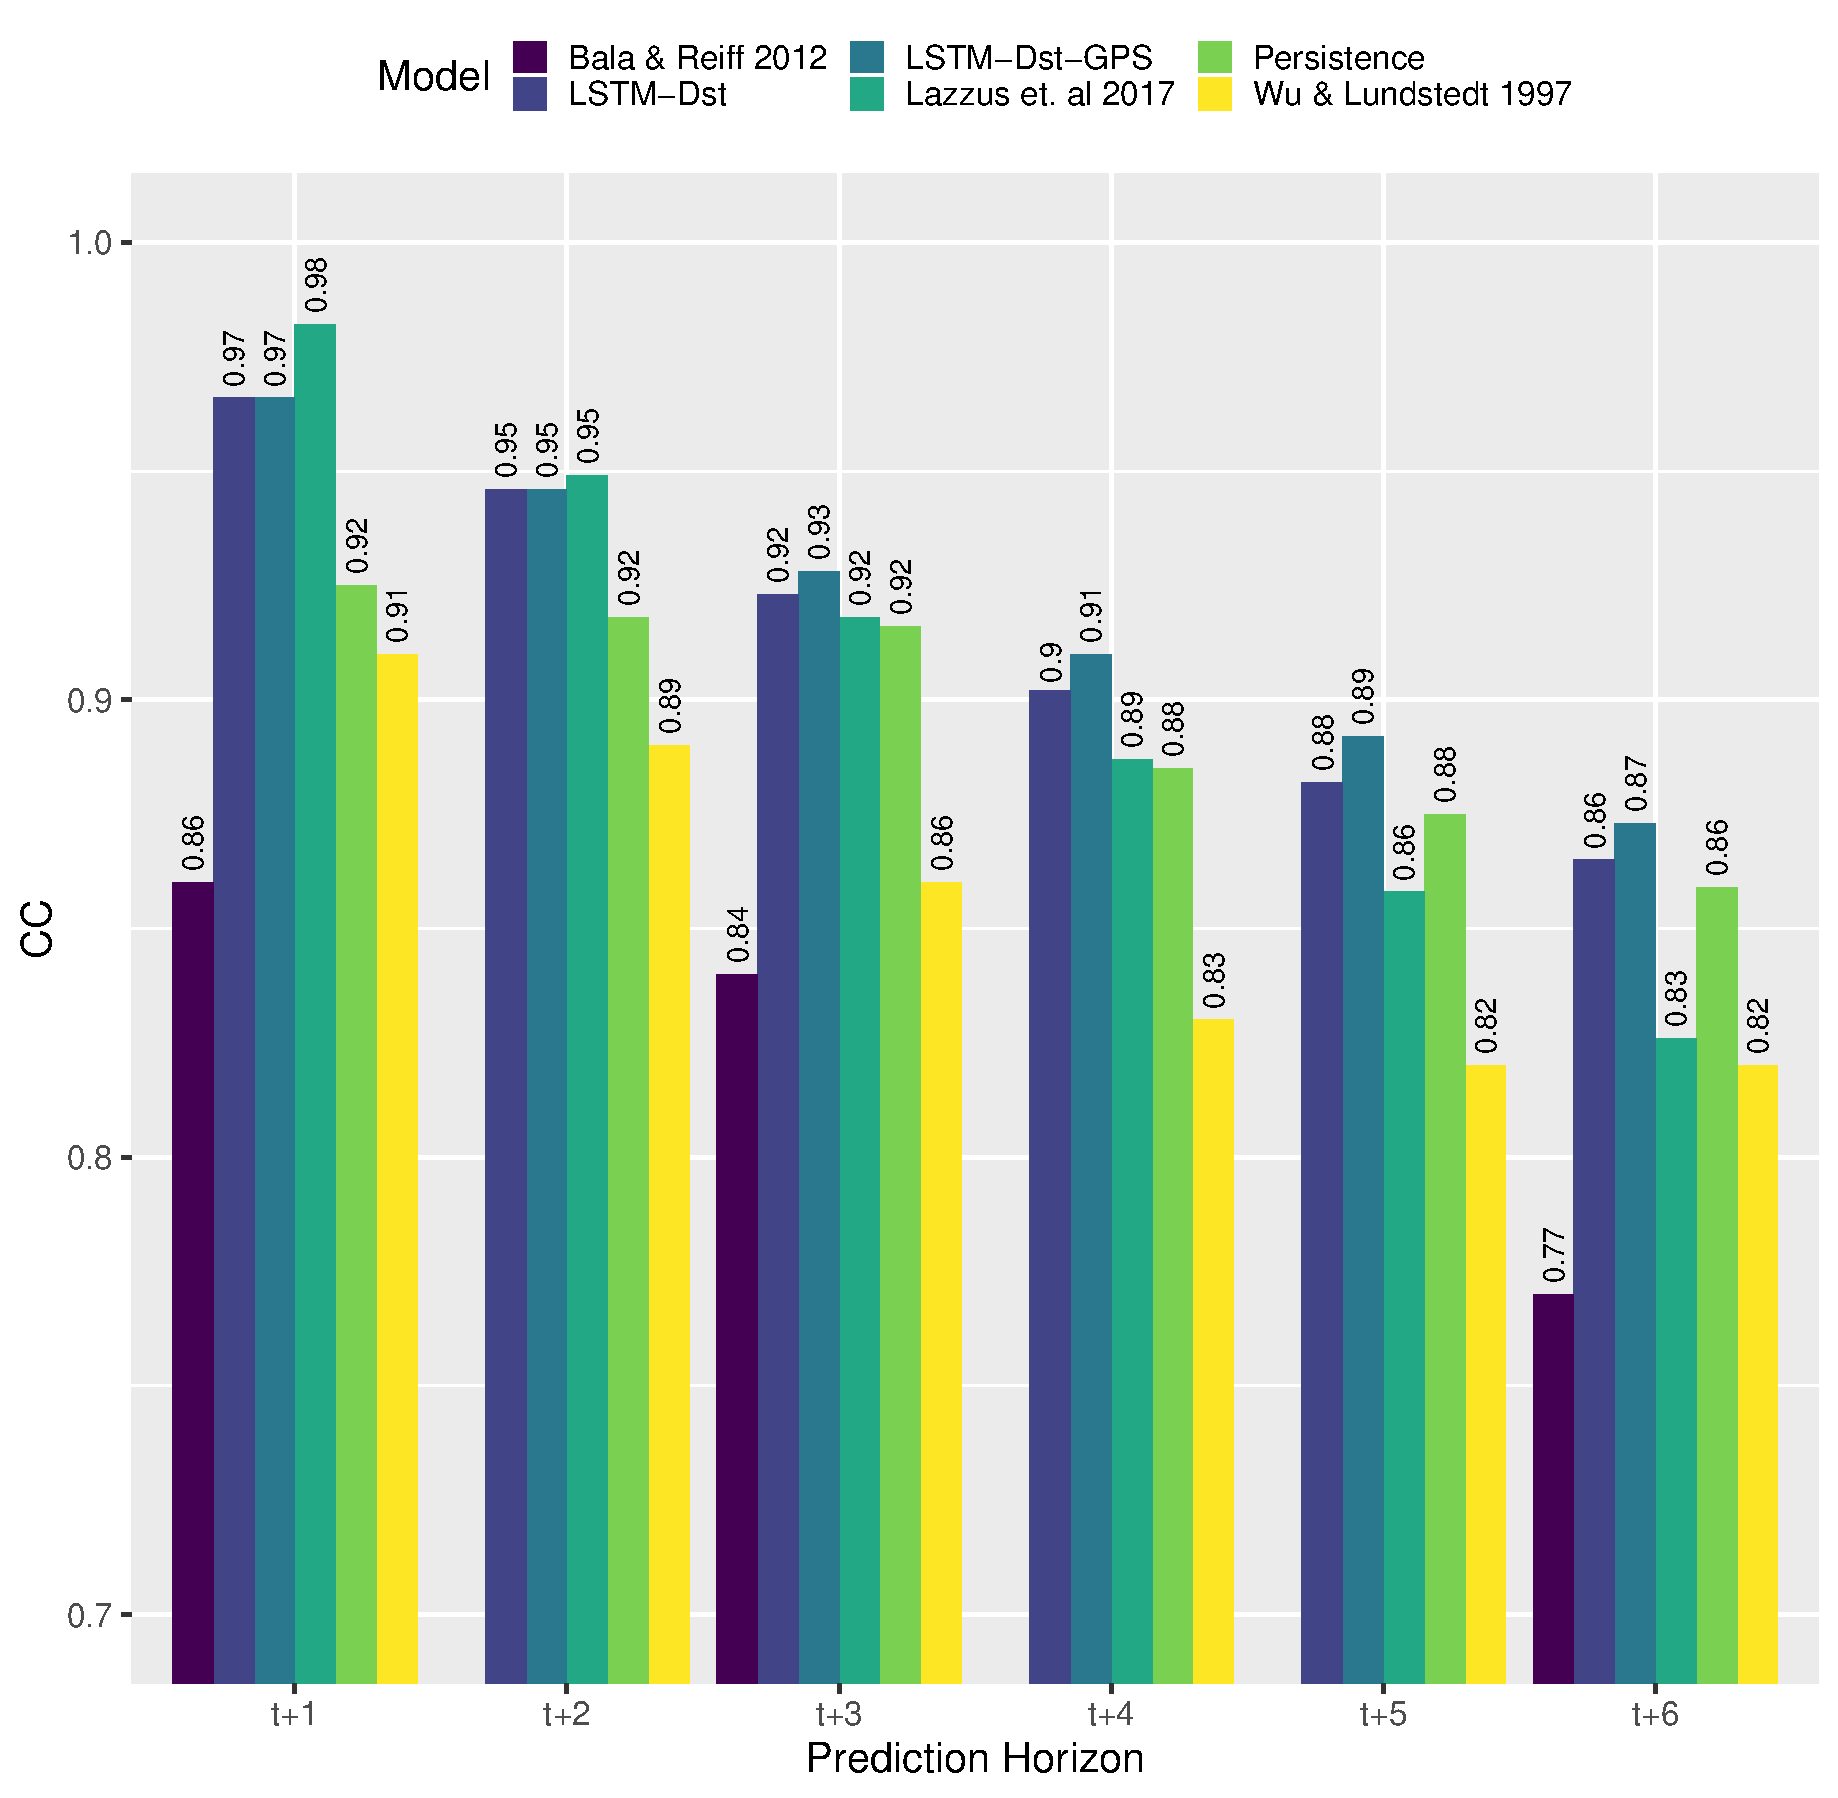
\includegraphics[width=\textwidth]{lstmCompCC.pdf}
	\caption{Comparison of CC of $Dst$ forecast models.}
	\label{fig:lstmCC}
\end{figure}


We wanted to compare the performance of a classic recurrent network to the LSTM, and see 
how the complexity of the LSTM cell could provide more accurate predictions. Wu and Lundstedt \citet{wu1997geomagnetic} 
provided for a 6h ahead forecast a CC of 0.82 and a RMSE of 20.8, showing in comparison to our model with or 
without GPS data, that the LSTM cell brings more accuracy. We observed that using GPS data generally results 
in an improvement when considering important geomagnetic storms. Figure 4 presents predictions obtained with 
the LSTM NN, with GPS data in blue and without GPS data in red, for Dst forecast from 1h ahead to 6h ahead, 
for the 2003 Halloween storm event (peak at -422 nT). Predictions for 1h to 2h ahead are very similar, but when 
we consider the forecast of 3h ahead, the model without GPS data predicts a peak of -348 nT while the model 
with the GPS data provides a prediction of -405 nT. 

For a forecast done 4h ahead, the model without GPS data 
provides a prediction of -335 nT and the one with GPS data, a forecast of -380 nT. For predictions done 5 h ahead, 
predicted peak values are quite the same. However, the 6h ahead forecast shows that a single point prediction 
provided by the NN is not good enough and offers a strong rationale to combine the NN performance with the 
GP model to obtain a probabilistic forecast. 


\subsection{Evaluation of the GPNN model}

As we described before, the GP process aim to provide not only a\ single\ point\ prediction,\ 
but also an asssociated  uncertainty. Metrics like RMSE and CC are defined for single point prediction 
and  are not adequate  to evaluate  probabilistic forecast.

\begin{table}[h]
	%\fontsize{8}{9.6}\selectfont
	\centering
	\caption{Storm Classification}
	\label{table:stormclass}
	\begin{tabular}{ccccc}
	\hline
	Level of Activity & Storm Classification \\ \hline
	Dst $> -50 nT$ & Moderate\\
	$-250 nT \leq $ Dst $\leq -50 nT$ & Intense\\
	Dst $\leq -250 nT$ & Super Storm\\ \hline
	\end{tabular}
\end{table}

Storm activity is often classified using given thresholds of Dst values. According to the most common 
classification, we distinguished 3 levels of storms summarised in Table \ref{table:stormclass} 
($\text{Dst} <= 250$, $-250 <= \text{Dst} <= 50$, $\text{Dst} >= -50$). The aim here is to use metrics 
which will be able to evaluate how the GPNN manages to forecast geomagnetic storms into the 
right family of storm. To do so, we focused on the Receiver Operating Characteristic Curve and 
Reliability diagram.



\subsubsection{Receiver Operating Characteristic Curve}


Our GPNN model provides to an operator a probabilistic forecast, which can be used in a decision-maing scenario. 
For example, a decision made by an operator to turn off a system according to the level of storm might be taken 
when the forecast probability of this storm exceeds a predetermined trigger threshold. For any storm, 
a Receiver Operating Characteristic Curve (ROC curve) can be constructed. 

This ROC curve is based on a contingency table in which predictions of Dst are classified according to the 
real value of Dst. The aim is to estimate the probability of a prediction to belong to the right category of storm 
via binary classification, in the sense one category versus all the others. Camporeale et al. (2017) used the 
same process to classify the category of solar events between ejecta, Coronal Hole, Sector reversal and streamer belt. 
The ROC curves represents the False Positive Ratio (FPR) versus the True Positive Ratio (TPR). The FPR is the ratio 
of false positive divided by the total number of negatives. The TPR also called sensitivity is the ratio of 
true positives divided by the total number of positives. For perfect classifications, the FPR has to be equal to 0 
and TPR equal to 1, thus the value of the threshold that produces the point closest to these values is optimal. 


Table 3 presents ROC values obtained from 1h to 6h ahead forecasts, depending on the level of the storm. 
The ROC is usually shown graphically, but numerical values are more relevant for the reader to analyse 
variations depending on the threshold. The optimal threshold is in red and bold, it is computed to 
minimise the Euclidean distance from FPR =0 and TPR =1. ROC values obtained for the highest level of activity, 
meaning Dst values<-250 nT provide FPR for each threshold 
(the highest value is $2.7.10^{-3}$ for a 10$\%$  threshold when considering a 1h forecast). 
The TPR behaviour is more complicated to generalise. For predictions done from 1h ahead to 5h ahead, 
values are always greater than 0.719 for thresholds from 10$\%$  to 40$\%$ , and then there is a decrease. 
If we focuse on the 6h ahead forecast, the best TPR is 0.5 for a 10$\%$  threshold. It means that the more 
there is an increasing probability for a superstorm to occur, the less the model is able to forecast it 
without misjudgements 6h in advance. However, for intense storms (-250 nT<Dst<-50 nT), the GPNN provides 
TPR higher than 0.670 for thresholds between 10$\%$  and 80$\%$ , and for moderate storms, this model provides 
TPR higher than 0.649 for every thresholds, from 1h to 6h ahead. 


\subsubsection{Reliability diagram}


The ROC discussed in the previous section gives information about the ability of the forecast system to 
detect the occurrence of a geomagnetic storm event for a given threshold, in terms of false and true positive. 
Reliability diagrams measure how closely the forecast probabilities of an event correspond to the actual 
frequency with which an event is observed. A perfectly reliable forecast is one in which an\ event\ predicted\ 
with probability p is observed, on average, with frequency p. The reliability diagram bins the forecasts into 
groups according to the issued probability, shown on the horizontal axis. The frequency with which an event was 
observed to occur for each bin is then plotted on the vertical axis.  If the reliability curve lies above/below 
than the perfect diagonal slope, the resulting forecasts  are under/over confident, i.e. they yield  
smaller/higher probabilities for a specific outcome than observed. 


Figure \ref{fig:gpnnreliability} presents reliability diagrams obtained from 1h to 6h ahead forecasts. 
It shows that the 1h ahead forecast slightly underestimates the storm, when there is more than 35$\%$  of 
probabilities for a given value of Dst. For example, when there is 80$\%$  of risk for a predicted storm, 
the real observed frequency of it is 90$\%$. The GPNN provides reliable forecast for 2h ahead prediction, 
as the observed frequency of storm regarding the predicted probability defines almost perfectly a diagonal. 
For predictions further than 3h ahead, the more it goes in time, the more it overestimates the probability of storms. 

If we focus on the 6h ahead prediciton, when the GPNN model provides a predicted probability of 90$\%$, the 
real observed frequency is of 65$\%$ . This model is over-confident. Once the reliability diagram is obtained, 
it is of interest to seek simple corrections to the forecast probabilities (re-calibration). This issue will be 
investigated elsewhere in greater detail. Here, we just show Figure \ref{fig:gpnnreliabilitysigma} that by multiplying 
the standard deviation by a\ factor of 2 or 3, it it possible to improve the reliability for predicted probability 
higher than 50$\%$ (Figure \ref{fig:gpnnreliability}). For example, if the predicted probability is 90$\%$, 
by multiplying sigma by 2, the corresponding real frequency is 72$\%$ and if we multiply by 3 we get 80$\%$. 
This way, we managed to get closer to the diagonal, when the probability of events increase. Conversely, 
a simple rescaling of the obtained standard deviation yields worse reliability for probabilities smaller than 50$\%$ .  


Figure \ref{fig:gpnnhalloween} presents predictions provided by the GPNN model for the 2003 Halloween storm. 
For predictions from 1h ahead to 5h ahead, thanks to this process, the predicted value of Dst is close to the 
real value. For example, for 5h ahead, the real peak of activity of -422 nT has a predicted value of -391 nT. 

The main contribution of the GP process here is shown for the 6h ahead forecast. While the LSTM alone failed to 
reach the highest peak of activity, the GPNN manages to have a predicted value closer to the real value than 
the LSTM one, and the covariance over the mean value encompasses the peak of activity.



\section{Conclusion}


In this paper, we have presented a model to predict the geomagnetic index Dst from 1h to 6h ahead, 
based on the combination of ANN and GP, called GPNN. 

First, we developed a \emph{long short-term memory} neural network, to provide Dst predictions from 1h to 6h ahead. 
A specific LSTM has been developed for each time predictions, then global performance of LSTM have been compared 
to past forecasting models of Dst. It shows that the LSTM provides very good global performance in comparison 
to previous models. When focusing on superstorm like the well known 2003 Halloween storm, we underlined that 
even if global metrics are excellent, the 6h ahead forecast fails to predict the highest peak of activity. 


Second, to obtain a probabilistic forecast instead of a single point prediction, we developed a GP which 
considers the LSTM as the mean function. Thanks to this combination, we observed that we managed to predict 
accurately superstorm like the 2003 Halloween storm for predictions from 1h ahead to 5h ahead. For the 
6h ahead prediction, the covariance manages to encompass the peak of activity. 

To evaluate this probabilistic forecast, we use ROC curves and reliability diagram. ROC curves demonstrate that, 
for each time forecast, storm level and threshold, the False Positive Ratio is very low. However, concerning 
True Positive Ratio, values are great for moderate and intense storms, but for 6h ahead prediction of superstorm, 
misjudgement is possible when the threshold increases. In this case, the optimal threshold is around 10$\%$ , 
which will need further improvement The reliability diagram shows that as the prediction goes further in time, 
the GPNN provides great performance for predictions from 1h to 3h ahead, but for 4h to 6h ahead, 
an overestimation of the storm is possible. We also demonstrate that thanks to this diagram, it is possible to 
evaluate the optimisation required to improve the reliability of the GPNN, and possibly to 
re-calibrate the prediction


\begin{table}[h]
	\centering
	\caption{ROC contingency table for the $t+1$ GPNN model.}
	\label{table:rocgpnn1h}
	\begin{tabular}{c| c c | c c | c c}
		\hline
		\multicolumn{7}{c}{\textbf{1‐hr‐ahead prediction}} \\ 
		\hline
		 & \multicolumn{2}{c}{\textit{Super Storm}} & \multicolumn{2}{c}{\textit{Intense Storm}} & \multicolumn{2}{c}{\textit{Moderate}} \\ 
		\hline
		\textbf{Threshold} & \textbf{TPR} & \textbf{FPR} & \textbf{TPR} & \textbf{FPR} & \textbf{TPR} & \textbf{FPR} \\ 
		\hline
		$10\%$ & $0.969$ & $2.70\times10^{-3}$ & $0.981$ & $0.163$ & $0.999$ &$ 0.434$ \\ 
		$20\%$ & $0.969$ & $1.11\times10^{-3}$ & $0.961$ & $0.105$ & $0.996$ & $0.321$ \\ 
		$30\%$ & $\mathbf{0.969}$ & $\mathbf{6.40\times10^{-4}}$ & $\mathbf{0.927}$ & $\mathbf{0.0719}$ & $0.991$ & $0.240$ \\ 
		$40\%$ & $0.969$ & $4.00\times10^{-4}$ & $0.895$ & $0.049$ & $0.984$ & $0.185$ \\ 
		$50\%$ & $0.844$ & $3.00\times10^{-4}$ & $0.855$ & $0.0270$ & $0.972$ & $0.138$ \\ 
		$60\%$ & $0.812$ & $2.78\times10^{-4}$ & $0.806$ & $0.0161$ & $0.951$ & $0.102$ \\ 
		$70\%$ & $0.656$ & $2.78\times10^{-4}$ & $0.753$ & $9.30.10^{-3}$ & $\mathbf{0.929}$ & $\mathbf{0.0705}$ \\ 
		$80\%$ & $0.625$ & $2.78\times10^{-4}$ & $0.670$ & $3.95.10^{-3}$ & $0.895$ & $0.0371$ \\ 
		$90\%$ & $0.468$ & $9.27\times10^{-5}$ & $0.554$ & $1.61.10^{-3}$ & $0.838$ & $0.0178$\\
		\hline
	\end{tabular}
	
\end{table}

\begin{table}[ht]
	\centering
	\caption{ROC contingency table for the $t+2$ GPNN model.}
	\label{table:rocgpnn2h}
	\begin{tabular}
		{c| c c | c c | c c}
		\hline
		\multicolumn{7}{c}{\textbf{2‐hr‐ahead prediction}} \\ 
		\hline
		 & \multicolumn{2}{c}{\textit{Super Storm}} & \multicolumn{2}{c}{\textit{Intense Storm}} & \multicolumn{2}{c}{\textit{Moderate}} \\ 
		\hline
		\textbf{Threshold} & \textbf{TPR} & \textbf{FPR} & \textbf{TPR} & \textbf{FPR} & \textbf{TPR} & \textbf{FPR} \\ 
		\hline
		$10\%$ & $0.969$ & $3.15\times10^{-3}$ & $0.963$ & $0.199$ & $0.999$ & $0.388$ \\ 
		$20\%$ & $0.937$ & $9.27\times10^{-4}$ & $0.934$ & $0.142$ & $0.984$ & $0.273$ \\ 
		$30\%$ & $\mathbf{0.937}$ & $\mathbf{3.71\times10^{-4}}$ & $\mathbf{0.914}$ & $\mathbf{0.105}$ & $0.973$ & $0.211$ \\ 
		$40\%$ & $0.906$ & $1.85\times10^{-4}$ & $0.891$ & $0.0834$ & $0.961$ & $0.167$ \\ 
		$50\%$ & $0.781$ & $1.85\times10^{-4}$ & $0.863$ & $0.0565$ & $0.943$ & $0.134$ \\ 
		$60\%$ & $0.6875$ & $9.27\times10^{-5}$ & $0.824$ & $0.0390$ & $\mathbf{0.917}$ & $\mathbf{0.107}$ \\ 
		$70\%$ & $0.656$ & $9.27\times10^{-5}$ & $0.783$ & $0.0268$ & $0.895$ & $0.0845$ \\ 
		$80\%$ & $0.500$ & $9.27\times10^{-5}$ & $0.720$ & $0.0156$ & $0.858$ & $0.0646$ \\ 
		$90\%$ & $0.437$ & $0$ & $0.601$ & 5.6810$^-3$ & $0.802$ & $0.0363$\\
		\hline
	\end{tabular}
\end{table}

\begin{table}[ht]
	\centering
	\caption{ROC contingency table for the $t+3$ GPNN model.}
	\label{table:rocgpnn3h}
	\begin{tabular}
		{c| c c | c c | c c}
		\hline
		\multicolumn{7}{c}{\textbf{3‐hr‐ahead prediction}} \\ 
		\hline
		 & \multicolumn{2}{c}{\textit{Super Storm}} & \multicolumn{2}{c}{\textit{Intense Storm}} & \multicolumn{2}{c}{\textit{Moderate}} \\ 
		\hline
		\textbf{Threshold} & \textbf{TPR} & \textbf{FPR} & \textbf{TPR} & \textbf{FPR} & \textbf{TPR} & \textbf{FPR} \\ 
		\hline
		$10\%$ & $0.875$ & $3.24\times10^{-3}$ & $0.958$ & $0.254$ & $0.984$ & $0.373$ \\ 
		$20\%$ & $\mathbf{0.843}$ & $\mathbf{9.27\times10^{-4}}$ & $0.939$ & $0.186$ & $0.971$ & $0.278$ \\ 
		$30\%$ & $0.813$ & $4.64\times10^{-4}$ & $0.912$ & $0.139$ & $0.955$ & $0.228$ \\ 
		$40\%$ & $0.750$ & $1.86\times10^{-4}$ & $\mathbf{0.890}$ & $\mathbf{0.106}$ & $0.940$ & $0.182$ \\ 
		$50\%$ & $0.625$ & $9.27\times10^{-5}$ & $0.880$ & $0.0819$ & $0.919$ & $0.146$ \\ 
		$60\%$ & $0.593$ & $0$ & $0.809$ & $0.0606$ & $\mathbf{0.893}$ & $\mathbf{0.1058}$ \\ 
		$70\%$ & $0.593$ & $0$ & $0.766$ & $0.0451$ & $0.826$ & $0.0865$ \\ 
		$80\%$ & $0.437$ & $0$ & $0.714$ & $0.0291$ & $0.814$ & $0.0594$ \\ 
		$90\%$ & $0.406$ & $0$ & $0.614$ & $0.0164$ & $0.747$ & $0.0413$\\
		\hline
	\end{tabular}
\end{table}


\begin{table}[ht]
	\centering
	\caption{ROC contingency table for the $t+4$ GPNN model.}
	\label{table:rocgpnn4h}
	\begin{tabular}
		{c| c c | c c | c c}
		\hline
		\multicolumn{7}{c}{\textbf{4‐hr‐ahead prediction}} \\ 
		\hline
		 & \multicolumn{2}{c}{\textit{Super Storm}} & \multicolumn{2}{c}{\textit{Intense Storm}} & \multicolumn{2}{c}{\textit{Moderate}} \\ 
		\hline
		\textbf{Threshold} & \textbf{TPR} & \textbf{FPR} & \textbf{TPR} & \textbf{FPR} & \textbf{TPR} & \textbf{FPR} \\ 
		\hline
		$10\%$ & $0.906$ & $3.24\times10^{-3}$ & $0.968$ & $0.311$ & $0.970$ & $0.339$ \\ 
		$20\%$ & $\mathbf{0.875}$ & $\mathbf{1.29\times10^{-3}}$ & $0.953$ & $0.252$ & $0.949$ & $0.243$ \\ 
		$30\%$ & $0.813$ & $7.42\times10^{-4}$ & $0.933$ & $0.208$ & $0.931$ & $0.192$ \\ 
		$40\%$ & $0.813$ & $6.49\times10^{-4}$ & $\mathbf{0.916}$ & $\mathbf{0.169}$ & $0.906$ & $0.144$ \\ 
		$50\%$ & $0.781$ & $9.27\times10^{-5}$ & $0.895$ & $0.138$ & $\mathbf{0.874}$ & $\mathbf{0.104}$ \\ 
		$60\%$ & $0.687$ & $9.27\times10^{-5}$ & $0.843$ & $0.106$ & $0.841$ & $0.0803$ \\ 
		$70\%$ & $0.562$ & $9.27\times10^{-5}$ & $0.795$ & $0.0812$ & $0.802$ & $0.0636$ \\ 
		$80\%$ & $0.468$ & $9.27\times10^{-5}$ & $0.742$ & $0.0621$ & $0.76$ & $0.0449$ \\ 
		$90\%$ & $0.437$ & $9.27\times10^{-5}$ & $0.640$ & $0.0403$ & $0.699$ & $0.0300$\\
		\hline
	\end{tabular}
\end{table}

\begin{table}[ht]
	\centering
	\caption{ROC contingency table for the $t+5$ GPNN model.}
	\label{table:rocgpnn5h}
	\begin{tabular}
		{c| c c | c c | c c}
		\hline
		\multicolumn{7}{c}{\textbf{5‐hr‐ahead prediction}} \\ 
		\hline
		 & \multicolumn{2}{c}{\textit{Super Storm}} & \multicolumn{2}{c}{\textit{Intense Storm}} & \multicolumn{2}{c}{\textit{Moderate}} \\ 
		\hline
		\textbf{Threshold} & \textbf{TPR} & \textbf{FPR} & \textbf{TPR} & \textbf{FPR} & \textbf{TPR} & \textbf{FPR} \\ 
		\hline
		$ 10\%$ & $ 0.812 $ & $3.06\times10^{-3}$ & $ 0.956 $ & $ 0.316 $ & $ 0.962 $ & $0.346$ \\ 
		$ 20\%$ & $\mathbf{0.812}$ & $\mathbf{1.02\times10^{-3}}$ & $ 0.934 $ & $ 0.246 $ & $ 0.945 $ & $0.265$ \\ 
		$ 30\%$ & $ 0.750 $ & $4.63\times10^{-4}$ & $ 0.917 $ & $ 0.189 $ & $ 0.926 $ & $0.215$ \\ 
		$ 40\%$ & $ 0.719 $ & $9.27\times10^{-5}$ & $ 0.891 $ & $ 0.148 $ & $ 0.906 $ & $0.171$ \\ 
		$ 50\%$ & $ 0.625 $ & $9.27\times10^{-5}$ & $\mathbf{0.856}$ & $\mathbf{0.120}$ & $ 0.881 $ & $0.139$ \\ 
		$ 60\%$ & $ 0.562 $ & $9.27\times10^{-5}$ & $ 0.824 $ & $ 0.0942 $ & $\mathbf{0.853}$ & $\mathbf{0.107}$ \\ 
		$ 70\%$ & $ 0.468 $ & $ 0 $ & $ 0.779 $ & $ 0.0740 $ & $ 0.810 $ & $0.081$ \\ 
		$ 80\%$ & $ 0.468 $ & $ 0 $ & $ 0.725 $ & $ 0.055 $ & $ 0.754 $ & $0.0654$ \\ 
		$ 90\%$ & $ 0.468 $ & $ 0 $ & $ 0.639 $ & $ 0.0381 $ & $ 0.685 $ & $0.0430$\\
		\hline
	\end{tabular}
\end{table}

\begin{table}[ht]
	\centering
	\caption{ROC contingency table for the $t+6$ GPNN model.}
	\label{table:rocgpnn6h}
	\begin{tabular}
		{c| c c | c c | c c}
		\hline
		\multicolumn{7}{c}{\textbf{5‐hr‐ahead prediction}} \\ 
		\hline
		 & \multicolumn{2}{c}{\textit{Super Storm}} & \multicolumn{2}{c}{\textit{Intense Storm}} & \multicolumn{2}{c}{\textit{Moderate}} \\ 
		\hline
		\textbf{Threshold} & \textbf{TPR} & \textbf{FPR} & \textbf{TPR} & \textbf{FPR} & \textbf{TPR} & \textbf{FPR} \\ 
		\hline
		$ 10\%$ & $\mathbf{0.500}$ & $\mathbf{8.34.10^{-3}}$ & $ 0.953 $ & $ 0.352 $ & $ 0.932 $ & $ 0.307 $ \\ 
		$ 20\%$ & $ 0.437 $ & $4.92\times10^{-3}$ & $ 0.928 $ & $ 0.289 $ & $ 0.909 $ & $ 0.241 $ \\ 
		$ 30\%$ & $ 0.437 $ & $3.24\times10^{-3}$ & $ 0.904 $ & $ 0.244 $ & $ 0.886 $ & $ 0.186 $ \\ 
		$ 40\%$ & $ 0.406 $ & $2.78\times10^{-3}$ & $ 0.890 $ & $ 0.202 $ & $ 0.862 $ & $ 0.161 $ \\ 
		$ 50\%$ & $ 0.375 $ & $1.76\times10^{-3}$ & $\mathbf{0.859}$ & $\mathbf{0.167}$ & $\mathbf{0.834}$ & $\mathbf{0.130}$\\ 
		$ 60\%$ & $ 0.375 $ & $1.39\times10^{-3}$ & $ 0.821 $ & $ 0.138 $ & $ 0.798 $ & $ 0.113 $ \\ 
		$ 70\%$ & $ 0.281 $ & $7.47\times10^{-4}$ & $ 0.788 $ & $ 0.115 $ & $ 0.757 $ & $ 0.0914 $ \\ 
		$ 80\%$ & $ 0.281 $ & $3.70\times10^{-4}$ & $ 0.735 $ & $ 0.0926 $ & $ 0.712 $ & $ 0.0693 $ \\ 
		$ 90\%$ & $ 0.281 $ & $2.78\times10^{-4}$ & $ 0.661 $ & $ 0.0691 $ & $ 0.649 $ & $ 0.0455 $ \\
		\hline
	\end{tabular}
\end{table}

%%%%%%%%%%%%%%%%%%%% Figure/Image No: 1 Ends here %%%%%%%%%%%%%%%%%%%%



%%%%%%%%%%%%%%%%%%%% Figure/Image No: 6 starts here %%%%%%%%%%%%%%%%%%%%

\begin{figure}
	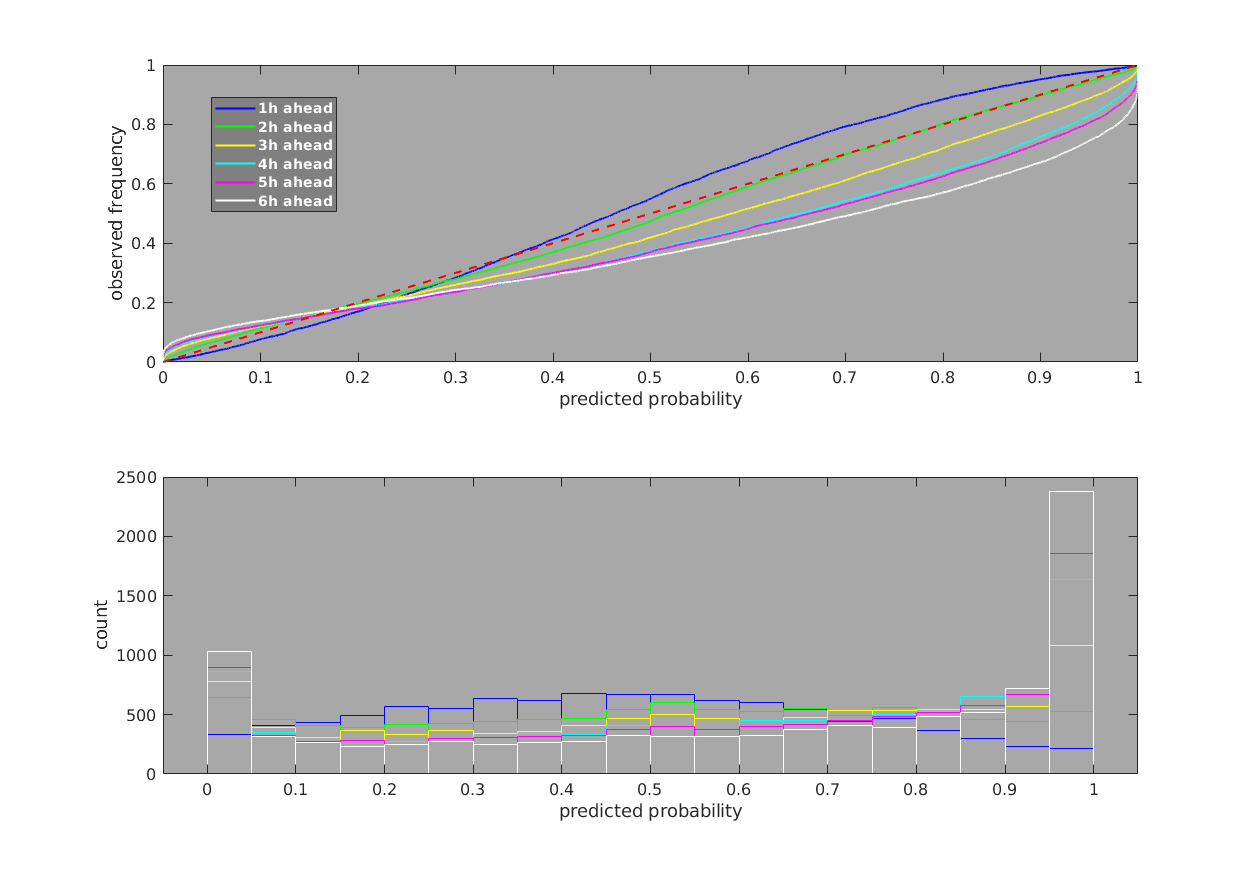
\includegraphics[width=\textwidth]{image6.png}
	\caption{Reliability diagram for Dst forecast from 1h ahead to 6h ahead. The diagonal is in red dot line.}
	\label{fig:gpnnreliability}
\end{figure}


%%%%%%%%%%%%%%%%%%%% Figure/Image No: 6 Ends here %%%%%%%%%%%%%%%%%%%%



%%%%%%%%%%%%%%%%%%%% Figure/Image No: 7 starts here %%%%%%%%%%%%%%%%%%%%

\begin{figure}
	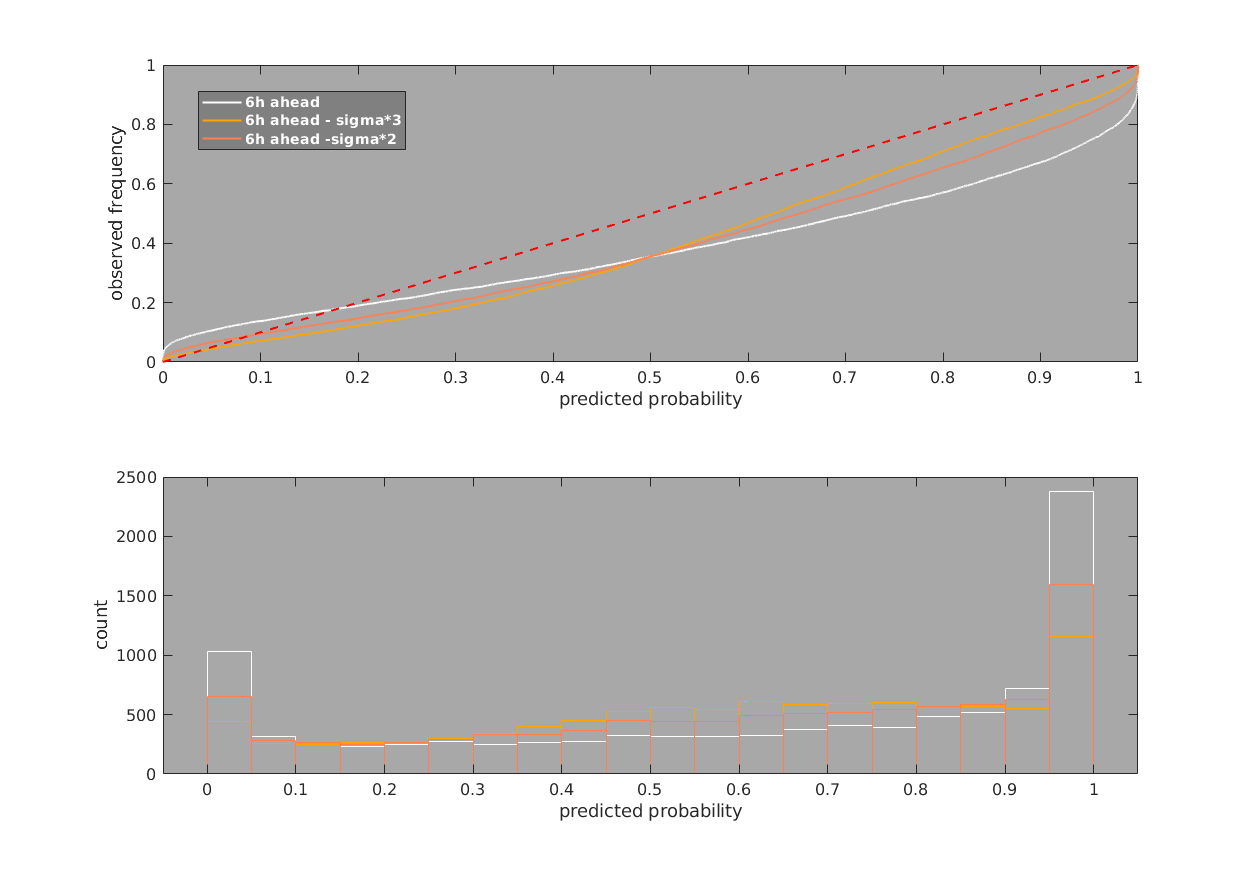
\includegraphics[width=\textwidth]{image7.png}
	\caption{Reliability diagram for the Dst prediction depending on the sigma value. The diagonal is in red dot line.}
	\label{fig:gpnnreliabilitysigma}	
\end{figure}


%%%%%%%%%%%%%%%%%%%% Figure/Image No: 7 Ends here %%%%%%%%%%%%%%%%%%%%

%%%%%%%%%%%%%%%%%%%% Figure/Image No: 8 starts here %%%%%%%%%%%%%%%%%%%%

\begin{figure}
	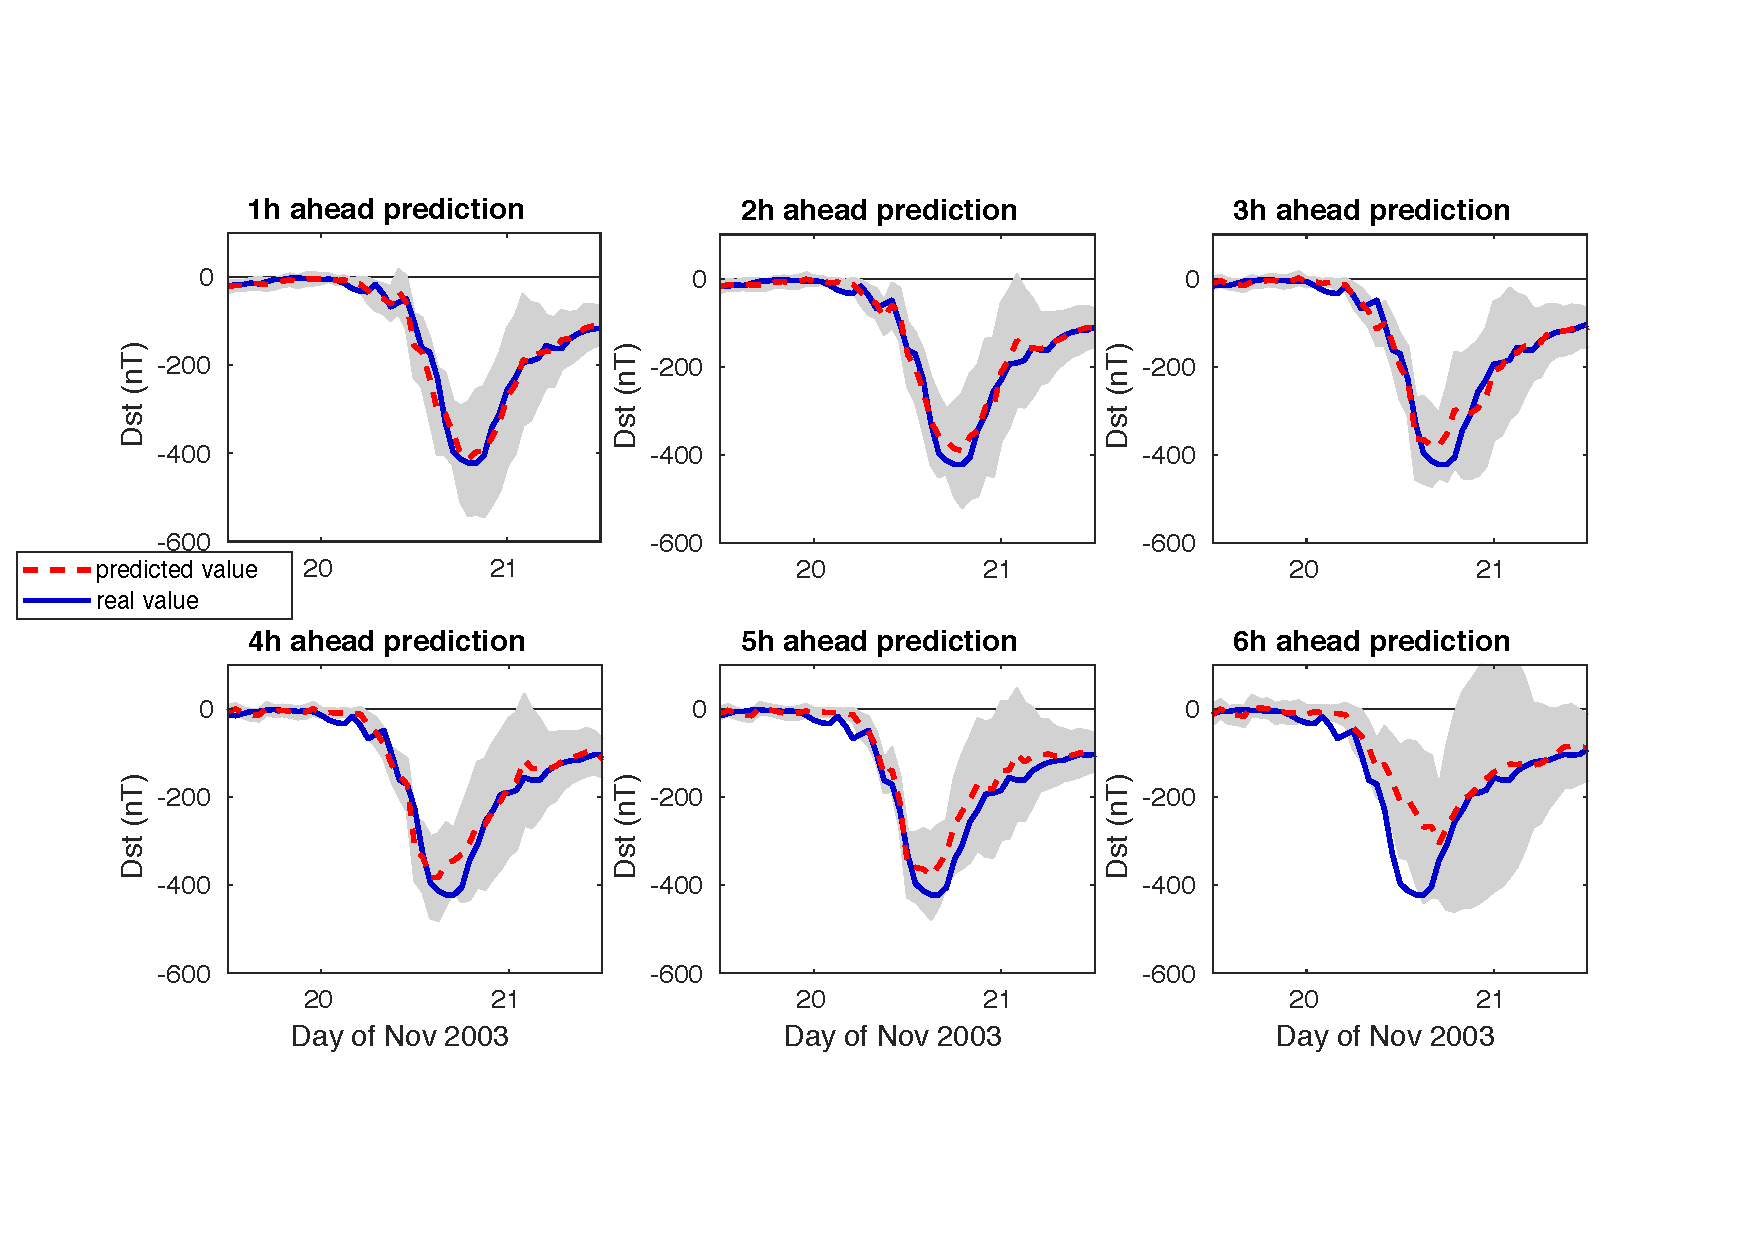
\includegraphics[width=\textwidth]{halloween_storm_GPNN.pdf}
	\caption{$Dst$ predictions made by the GPNN for the 2003 Halloween storm. 
	The most probable prediction is the dotted purple line. 
	The ground truth $Dst$ is the deep blue line. 
	The grey shadow represents $\pm\sigma$ error bars on the prediction.}
    \label{fig:gpnnhalloween}
\end{figure}


%%%%%%%%%%%%%%%%%%%% Figure/Image No: 8 Ends here %%%%%%%%%%%%%%%%%%%%


\begin{table}[h]
	\fontsize{8}{9.6}\selectfont
	\centering
	\caption{Storm events used to evaluate GPNN model}
	\label{table:teststormsgpnn}
	\begin{tabular}{ccccc}
	\hline
	Start Date & Start Time & End Date & End Time & min. Dst \\ \hline
	2001/03/19 & 15:00 & 2001/03/21 & 23:00 & $ -149 $ \\
	2001/03/31 & 04:00 & 2001/04/01 & 21:00 & $ -387 $ \\
	2001/04/18 & 01:00 & 2001/04/18 & 13:00 & $ -114 $ \\
	2001/04/22 & 02:00 & 2001/04/23 & 15:00 & $ -102 $ \\
	2001/08/17 & 16:00 & 2001/08/18 & 16:00 & $ -105 $ \\
	2001/09/30 & 23:00 & 2001/10/02 & 00:00 & $ -148 $ \\
	2001/10/21 & 17:00 & 2001/10/24 & 11:00 & $ -187 $ \\
	2001/10/28 & 03:00 & 2001/10/29 & 22:00 & $ -157 $ \\
	2002/03/23 & 14:00 & 2002/03/25 & 05:00 & $ -100 $ \\
	2002/04/17 & 11:00 & 2002/04/19 & 02:00 & $ -127 $ \\
	2002/04/19 & 09:00 & 2002/04/21 & 06:00 & $ -149 $ \\
	2002/05/11 & 10:00 & 2002/05/12 & 16:00 & $ -110 $ \\
	2002/05/23 & 12:00 & 2002/05/24 & 23:00 & $ -109 $ \\
	2002/08/01 & 23:00 & 2002/08/02 & 09:00 & $ -102 $ \\
	2002/09/04 & 01:00 & 2002/09/05 & 00:00 & $ -109 $ \\
	2002/09/07 & 14:00 & 2002/09/08 & 20:00 & $ -181 $ \\
	2002/10/01 & 06:00 & 2002/10/03 & 08:00 & $ -176 $ \\
	2002/11/20 & 16:00 & 2002/11/22 & 06:00 & $ -128 $ \\
	2003/05/29 & 20:00 & 2003/05/30 & 10:00 & $ -144 $ \\
	2003/06/17 & 19:00 & 2003/06/19 & 03:00 & $ -141 $ \\
	2003/07/11 & 15:00 & 2003/07/12 & 16:00 & $ -105 $ \\
	2003/08/17 & 18:00 & 2003/08/19 & 11:00 & $ -148 $ \\
	2003/11/20 & 12:00 & 2003/11/22 & 00:00 & $ -422 $ \\
	2004/01/22 & 03:00 & 2004/01/24 & 00:00 & $ -149 $ \\
	2004/02/11 & 10:00 & 2004/02/12 & 00:00 & $ -105 $ \\
	2004/04/03 & 14:00 & 2004/04/04 & 08:00 & $ -112 $ \\
	2004/07/22 & 20:00 & 2004/07/23 & 20:00 & $ -101 $ \\
	2004/07/24 & 21:00 & 2004/07/26 & 17:00 & $ -148 $ \\
	2004/07/26 & 22:00 & 2004/07/30 & 05:00 & $ -197 $ \\
	2004/08/30 & 05:00 & 2004/08/31 & 21:00 & $ -126 $ \\
	2004/11/11 & 22:00 & 2004/11/13 & 13:00 & $ -109 $ \\
	2005/01/21 & 18:00 & 2005/01/23 & 05:00 & $ -105 $ \\
	2005/05/07 & 20:00 & 2005/05/09 & 10:00 & $ -127 $ \\
	2005/05/29 & 22:00 & 2005/05/31 & 08:00 & $ -138 $ \\
	2005/06/12 & 17:00 & 2005/06/13 & 19:00 & $ -106 $ \\
	2005/08/31 & 12:00 & 2005/09/01 & 12:00 & $ -131 $ \\
	2006/04/13 & 20:00 & 2006/04/14 & 23:00 & $ -111 $ \\
	2006/12/14 & 21:00 & 2006/12/16 & 03:00 & $ -147 $ \\ 
	2011/09/26 & 14:00 & 2011/09/27 & 12:00 & $ -101 $ \\
	2011/10/24 & 20:00 & 2011/10/25 & 14:00 & $ -132 $ \\
	2012/03/08 & 12:00 & 2012/03/10 & 16:00 & $ -131 $ \\
	2012/04/23 & 11:00 & 2012/04/24 & 13:00 & $ -108 $ \\
	2012/07/15 & 01:00 & 2012/07/16 & 23:00 & $ -127 $ \\
	2012/09/30 & 13:00 & 2012/10/01 & 18:00 & $ -119 $ \\
	2012/10/08 & 02:00 & 2012/10/09 & 17:00 & $ -105 $ \\
	2012/11/13 & 18:00 & 2012/11/14 & 18:00 & $ -108 $ \\
	2013/03/17 & 07:00 & 2013/03/18 & 10:00 & $ -132 $ \\
	2013/05/31 & 18:00 & 2013/06/01 & 20:00 & $ -119 $ \\
	2014/02/18 & 15:00 & 2014/02/19 & 16:00 & $ -112 $ \\ \hline
	\end{tabular}%
	\end{table}

	


%\bibliographystyle{plainnat}
%\bibliography{references}